\subsection{Premi::\gls{Back-End}}
	\subsubsection*{Informazioni sul package}
		\begin{figure}[h]
			\centering
			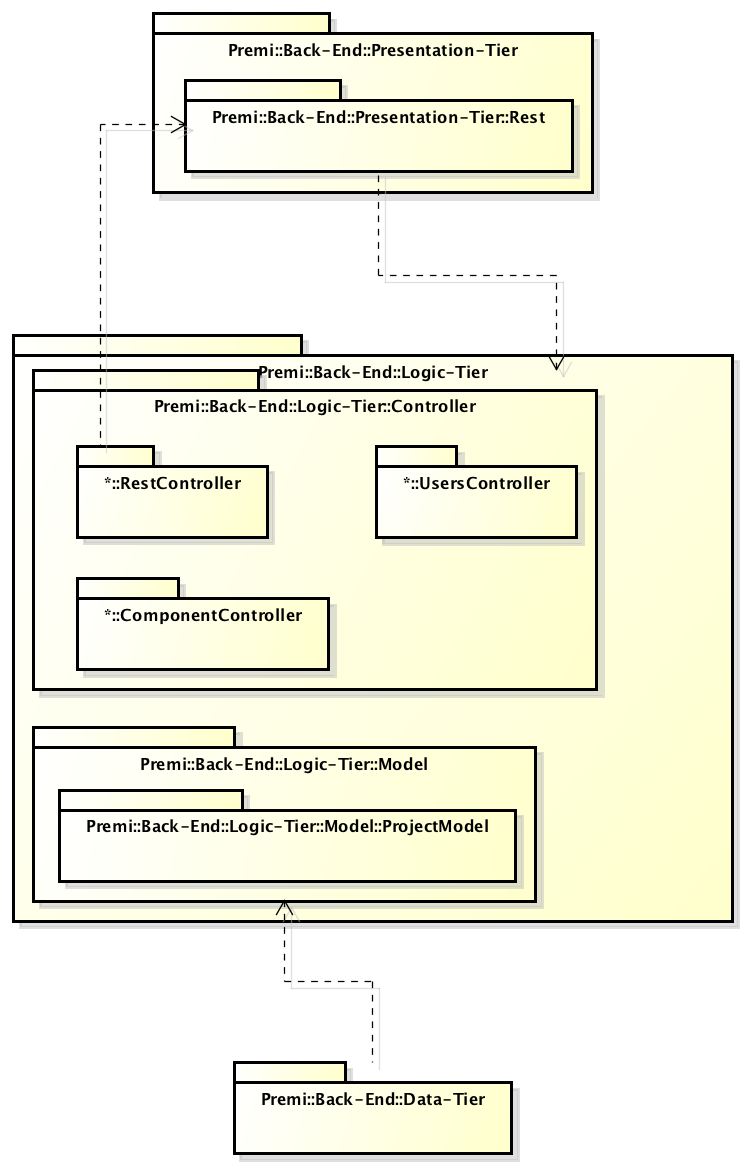
\includegraphics[width=0.7\linewidth]{img/back-end_package}
			\caption[Premi::Back-End]{Premi::Back-End}
		\end{figure}
		Il package contiene le componenti della parte di \gls{back-end} dell'applicazione.
		
	\subsubsection*{Package contenuti}
		\begin{itemize}
			\item Premi::\gls{Back-End}::Presentation-Tier;
			\item Premi::\gls{Back-End}::Logic-Tier;
			\item Premi::\gls{Back-End}::Data-Tier.
		\end{itemize}

\newpage

\subsection{Premi::Back-End::Presentation-Tier}
	\subsubsection*{Informazioni sul package}
		\begin{figure}[h]
			\centering
			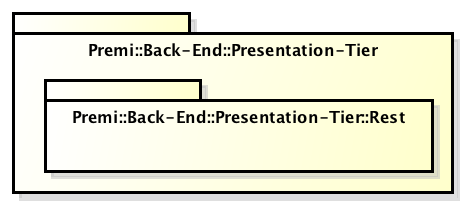
\includegraphics[width=0.5\linewidth]{img/back-end_presentation-tier}
			\caption[Premi::Back-End::Presentation-Tier]{Premi::Back-End::Presentation-Tier}
		\end{figure}
		Il package contiene le componenti necessarie per consentire il funzionamento del servizio \gls{REST}, in modo tale da rendere possibile l'interfacciamento con il \gls{front-end}.
		
	\subsubsection*{Package contenuti}
		\begin{itemize}
			\item Premi::Back-End::Data-Tier::REST:
			\begin{itemize}
				\item \textbf{Descrizione}: Il package contiene la struttura necessaria al funzionamento delle chiamate \gls{REST} da parte del \gls{front-end}, richiamando i rispettivi controller.
			\end{itemize}
		\end{itemize}
		
\newpage
		
\subsection{Premi::Back-End::Logic-Tier}
	\subsubsection*{Informazioni sul package}
	\begin{figure}[h]
		\centering
		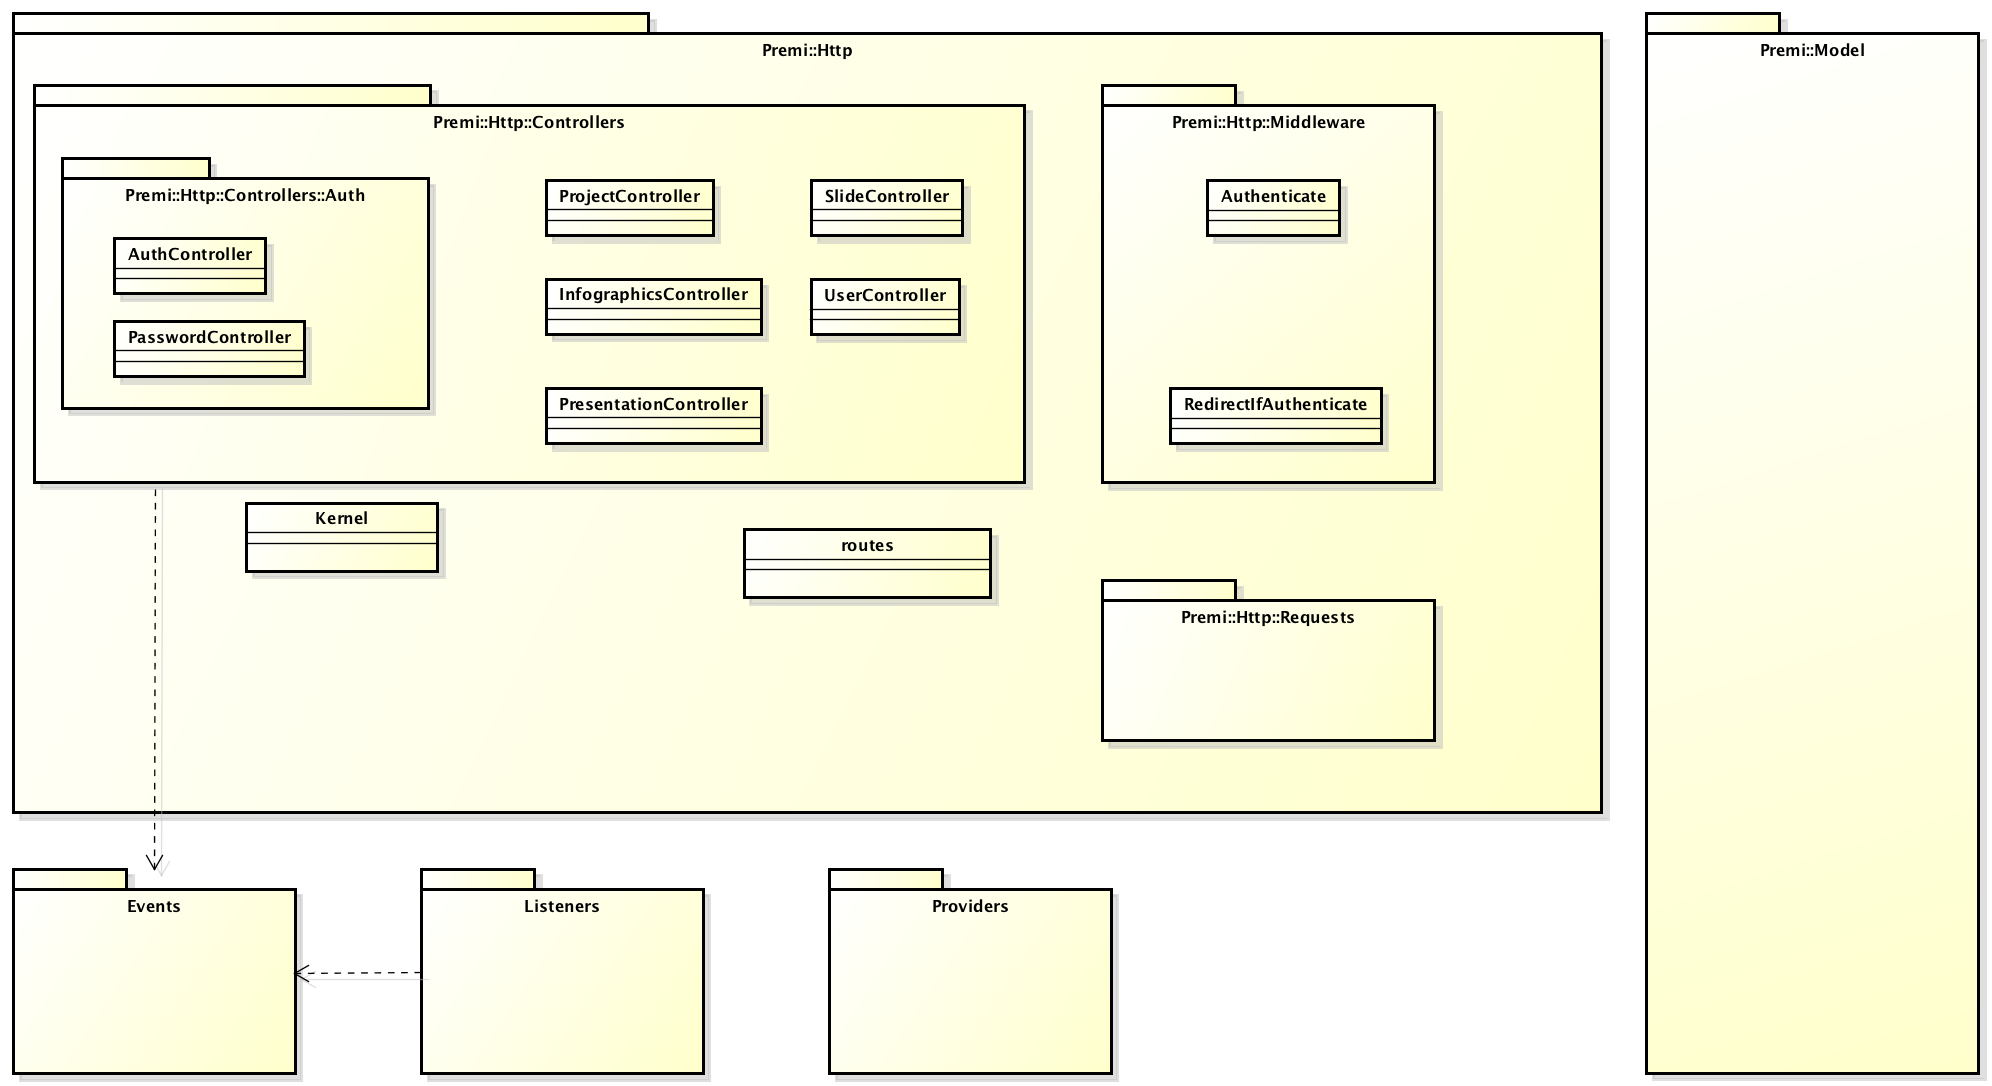
\includegraphics[width=0.9\linewidth]{img/back-end_logic-tier_package}
		\caption[Premi::Back-End::Logic-Tier]{Premi::Back-End::Logic-Tier}
	\end{figure}
	Il package contiene le componenti che si occupano di ricevere le richieste dal Presentation-Tier e di elaborarle attraverso il controller.
	
	\subsubsection*{Package contenuti}
	\begin{itemize}
		\item Premi::Back-End::Logic-Tier::Controller;
		\item Premi::Back-End::Logic-Tier::Model.
	\end{itemize}

\newpage

\subsection{Premi::Back-End::Logic-Tier::Controller}
	\subsubsection*{Informazioni sul package}
	\begin{figure}[h]
		\centering
		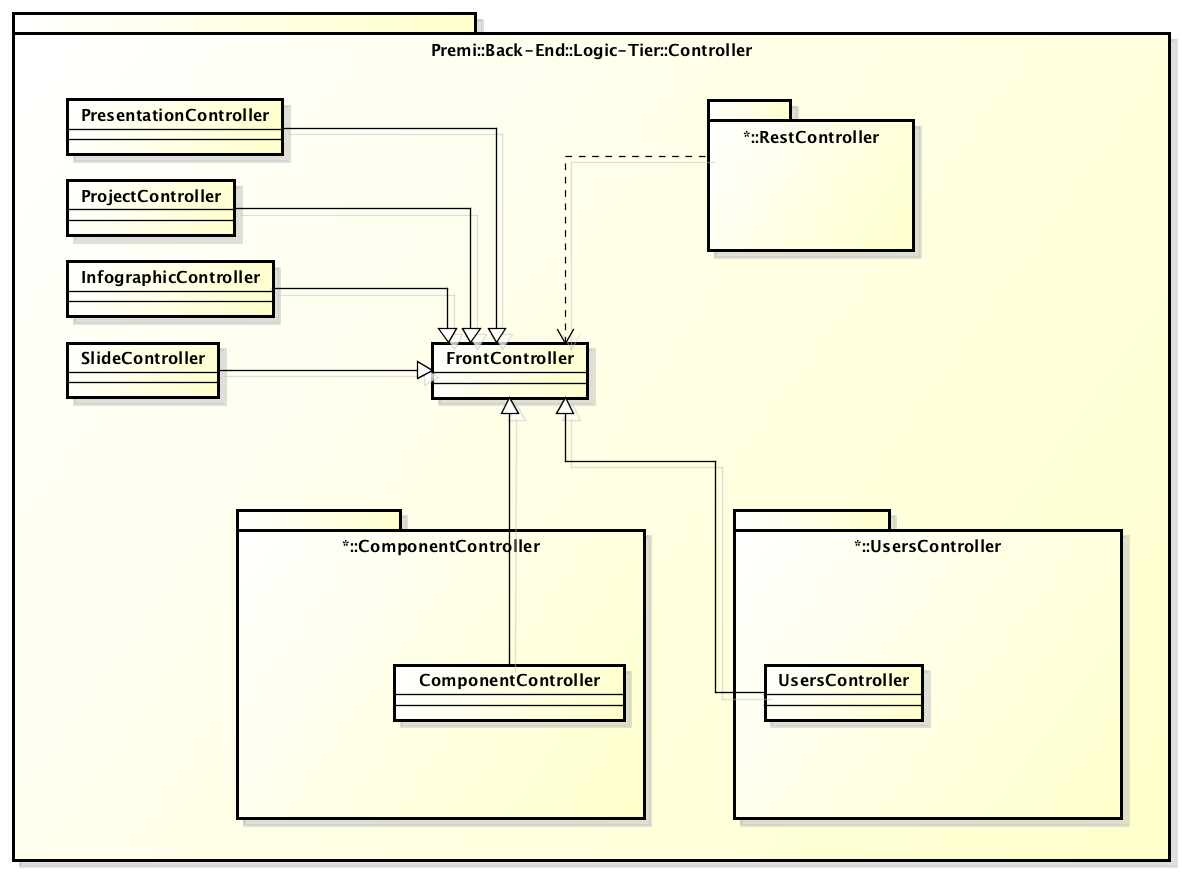
\includegraphics[width=0.9\linewidth]{img/back-end_logic-tier_controller}
		\caption[Premi::Back-End::Logic-Tier::Controller]{Premi::Back-End::Logic-Tier::Controller}
	\end{figure}
	Il package contiene le componenti che gestiscono la parte controller del lato \gls{back-end} dell'applicazione. Al suo interno è presente l'interfaccia comune \textit{FrontController} dalla quale derivano tutti i controller del programma.
	Sono presenti i controller per il progetto e i suoi componenti.

	\subsubsection*{Package contenuti}
		\begin{itemize}
			\item Premi::Back-End::Logic-Tier::Controller::ComponentController:
			\begin{itemize}
				\item Descrizione: Il package contiene i controller per la gestione degli elementi di una \gls{slide}.
			\end{itemize}
			
			\item Premi::Back-End::Logic-Tier::Controller::RestController:
			\begin{itemize}
				\item Descrizione: Il package contiene i controller per il \gls{REST}.
			\end{itemize}
			
			\item Premi::Back-End::Logic-Tier::Controller::UsersController:
			\begin{itemize}
				\item Descrizione: Il package contiene gli elementi di controller per la gestione delle funzioni per l'utente, come login, registrazione, ricerca, ecc.
			\end{itemize}
		\end{itemize}
		
	\subsubsection*{Classi contenute}
		\begin{itemize}
			\item Premi::Back-End::Logic-Tier::Controller::FrontController:
			\begin{itemize}
				\item \textbf{Descrizione}: Classe che gestisce le operazioni e la logica applicativa degli elementi del progetto.
				\item \textbf{Relazioni con altri package}:
				\begin{itemize}
					\item Premi::Back-End::Presentation-Tier::\gls{Rest}.
				\end{itemize}
			\end{itemize}
			
			\item Premi::Back-End::Logic-Tier::Controller::ProjectController:
			\begin{itemize}
				\item \textbf{Descrizione}: Classe che gestisce le operazioni e la logica riguardante la gestione e la modifica di un progetto;
				\item \textbf{Relazioni con altre classi}:
				\begin{itemize}
					\item Premi::Back-End::Logi-Tier::Controller::FrontController.
				\end{itemize}
			\end{itemize}
			
			\item Premi::Back-End::Logic-Tier::Controller::PresentationController:
			\begin{itemize}
				\item \textbf{Descrizione}: Classe che gestisce le operazioni e la logica riguardante la gestione e la modifica di una presentazione;
				\item \textbf{Relazioni con altre classi}:
				\begin{itemize}
					\item Premi::Back-End::Logi-Tier::Controller::FrontController.
				\end{itemize}
			\end{itemize}
			
			\item Premi::\gls{Back-End}::Logic-Tier::Controller::InfographicController:
			\begin{itemize}
				\item \textbf{Descrizione}: Classe che gestisce le operazioni e la logica riguardante la gestione e la modifica di un'\gls{infografica};
				\item \textbf{Relazioni con altre classi}:
				\begin{itemize}
					\item Premi::Back-End::Logi-Tier::Controller::FrontController.
				\end{itemize}
			\end{itemize}
			
			\item Premi::Back-End::Logic-Tier::Controller::SlideController:
			\begin{itemize}
				\item \textbf{Descrizione}: classe che gestisce le operazioni e la logica riguardante la gestione e la modifica di una \gls{slide};
				\item \textbf{Relazioni con altre classi}:
				\begin{itemize}
					\item Premi::Back-End::Logi-Tier::Controller::FrontController.
				\end{itemize}
			\end{itemize}
		\end{itemize}
		
\newpage
	
\subsection{Premi::Back-End::Logic-Tier::Controller::ComponentController}
	\subsubsection*{Informazioni sul package}
		\begin{figure}[h]
			\centering
			\includegraphics[width=0.9\linewidth]{img/back-end_logic-tier_controller_componentcontroller}
			\caption[Premi::Back-End::Logic-Tier::Controller::ComponentController]{Premi::Back-End::Logic-Tier::Controller::ComponentController}
		\end{figure}
		Il package contiene le classi dei controller per la gestione degli elementi di una \gls{slide}.
		
	\subsubsection*{Classi contenute}
	\begin{itemize}
		\item Premi::Back-End::Logic-Tier::Controller::ComponentController::ComponentController:
		\begin{itemize}
			\item \textbf{Descrizione}: classe che gestisce le operazioni e la logica applicativa di tutti i componenti della \gls{slide};
			\item \textbf{Relazioni con altre classi}:
			\begin{itemize}
				\item Premi::Back-End::Logic-Tier::Controller::FrontController.
			\end{itemize}
		\end{itemize}
		
		\item Premi::Back-End::Logic-Tier::Controller::ComponentController::RealTimeDataController:
		\begin{itemize}
			\item \textbf{Descrizione}: classe che gestisce le operazioni e la logica applicativa dei componenti per i dati real-time della \gls{slide};
			\item \textbf{Relazioni con altre classi}:
			\begin{itemize}
				\item Premi::Back-End::Logic-Tier::Controller::ComponentController::ComponentController.
			\end{itemize}
		\end{itemize}
		
		\item Premi::Back-End::Logic-Tier::Controller::ComponentController::ChartController:
		\begin{itemize}
			\item \textbf{Descrizione}: classe che gestisce le operazioni e la logica applicativa dei componenti per i grafici della \gls{slide};
			\item \textbf{Relazioni con altre classi}:
			\begin{itemize}
				\item Premi::Back-End::Logic-Tier::Controller::ComponentController::ComponentController.
			\end{itemize}
		\end{itemize}
		
		\item Premi::Back-End::Logic-Tier::Controller::ComponentController::ImageController:
		\begin{itemize}
			\item \textbf{Descrizione}: classe che gestisce le operazioni e la logica applicativa dei componenti per le immagini della \gls{slide};
			\item \textbf{Relazioni con altre classi}:
			\begin{itemize}
				\item Premi::Back-End::Logic-Tier::Controller::ComponentController::ComponentController.
			\end{itemize}
		\end{itemize}
		
		\item Premi::Back-End::Logic-Tier::Controller::ComponentController::TableController:
		\begin{itemize}
			\item \textbf{Descrizione}: classe che gestisce le operazioni e la logica applicativa dei componenti per le tabelle della \gls{slide};
			\item \textbf{Relazioni con altre classi}:
			\begin{itemize}
				\item Premi::Back-End::Logic-Tier::Controller::ComponentController::ComponentController.
			\end{itemize}
		\end{itemize}
		
		\item Premi::Back-End::Logic-Tier::Controller::ComponentController::TextController:
		\begin{itemize}
			\item \textbf{Descrizione}: classe che gestisce le operazioni e la logica applicativa dei componenti per le caselle di testo della \gls{slide};
			\item \textbf{Relazioni con altre classi}:
			\begin{itemize}
				\item Premi::Back-End::Logic-Tier::Controller::ComponentController::ComponentController.
			\end{itemize}
		\end{itemize}
	\end{itemize}
	
\newpage
	
\subsection{Premi::Back-End::Logic-Tier::Controller::UsersController}
	\subsubsection*{Informazioni sul package}
		\begin{figure}[h]
			\centering
			\includegraphics[width=0.9\linewidth]{img/back-end_logic-tier_controller_userscontroller}
			\caption[Premi::Back-End::Logic-Tier::Controller::UsersController]{Premi::Back-End::Logic-Tier::Controller::UsersController}
		\end{figure}
	Il package contiene le classi dei controller per la gestione degli utenti e le loro informazioni.
	
	\subsubsection*{Classi contenute}
		\begin{itemize}
			\item Premi::Back-End::Logic-Tier::Controller::UsersController::UsersController:
			\begin{itemize}
				\item \textbf{Descrizione}: classe che gestisce le operazioni e la logica applicativa di tutte le funzioni per la gestione di un utente e dei suoi dati;
				\item \textbf{Relazioni con altre classi}:
				\begin{itemize}
					\item Premi::Back-End::Logic-Tier::Controller::FrontController;
					\item Premi::Back-End::Logic-Tier::Model::User.
				\end{itemize}
			\end{itemize}
			
			\item Premi::Back-End::Logic-Tier::Controller::UsersController::LoginController:
			\begin{itemize}
				\item \textbf{Descrizione}: classe che gestisce le operazioni e la logica applicativa delle funzioni per il login di utente;
				\item \textbf{Relazioni con altre classi}:
				\begin{itemize}
					\item Premi::Back-End::Logic-Tier::Controller::UsersController::UsersController.
				\end{itemize}
			\end{itemize}
			
			\item Premi::Back-End::Logic-Tier::Controller::UsersController::ForgotPasswordController:
			\begin{itemize}
				\item \textbf{Descrizione}: classe che gestisce le operazioni e la logica applicativa per il recupero della password di un utente;
				\item \textbf{Relazioni con altre classi}:
				\begin{itemize}
					\item Premi::Back-End::Logic-Tier::Controller::UsersController::UsersController.
				\end{itemize}
			\end{itemize}
			
			\item Premi::Back-End::Logic-Tier::Controller::UsersController::RegistrationController:
			\begin{itemize}
				\item \textbf{Descrizione}: classe che gestisce le operazioni e la logica applicativa delle funzioni per la registrazione di un nuovo utente;
				\item \textbf{Relazioni con altre classi}:
				\begin{itemize}
					\item Premi::Back-End::Logic-Tier::Controller::UsersController::UsersController.
				\end{itemize}
			\end{itemize}
			
			\item Premi::Back-End::Logic-Tier::Controller::UsersController::SearchResultController:
			\begin{itemize}
				\item \textbf{Descrizione}: classe che gestisce le operazioni e la logica applicativa delle funzioni per la ricerca e la gestione dei risultati;
				\item \textbf{Relazioni con altre classi}:
				\begin{itemize}
					\item Premi::Back-End::Logic-Tier::Controller::UsersController::UsersController.
				\end{itemize}
			\end{itemize}
		\end{itemize}

\newpage

\subsection{Premi::Back-End::Logic-Tier::Model}
	\subsubsection*{Informazioni sul package}
		\begin{figure}[h]
			\centering
			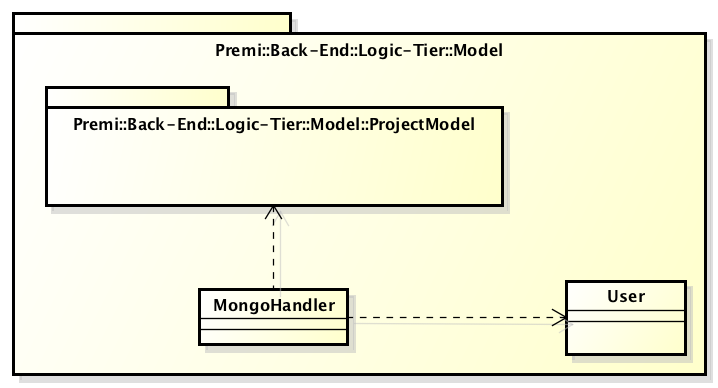
\includegraphics[width=0.9\linewidth]{img/back-end_logic-tier_model}
			\caption[Premi::Back-End::Logic-Tier::Model]{Premi::Back-End::Logic-Tier::Model}
		\end{figure}
		Il package contiene le classi che definisco il modello dell'applicazione.
	
	\subsubsection*{Package Contenuti}
		\begin{itemize}
			\item Premi::Back-End::Logic-Tier::Model::ProjectModel.
		\end{itemize}
	
	\subsubsection*{Classi contenute}
	\begin{itemize}
		\item Premi::Back-End::Logic-Tier::Model::MongoHandler:
		\begin{itemize}
			\item \textbf{Descrizione}: classe per comunicare con il livello inferiore ed interagire direttamente con la base di dati;
			\item \textbf{Relazione con altre classi}:
			\begin{itemize}
				\item Premi::Back-End::Logic-Tier::Controller::UsersController::UserController.
			\end{itemize}
		\end{itemize}
			
		\item Premi::Back-End::Logic-Tier::Model::Utente:
		\begin{itemize}
			\item \textbf{Descrizione}: classe che fornisce le operazioni per gestire un utente;
			\item \textbf{Relazione con altre classi}:
			\begin{itemize}
				\item Premi::Back-End::Data-Tier::DataTierFrontController.
			\end{itemize}
		\end{itemize}
	\end{itemize}

\newpage

\subsection{Premi::Back-End::Logic-Tier::Model::ProjectModel}
	\subsubsection*{Informazioni sul package}
		\begin{figure}[h]
			\centering
			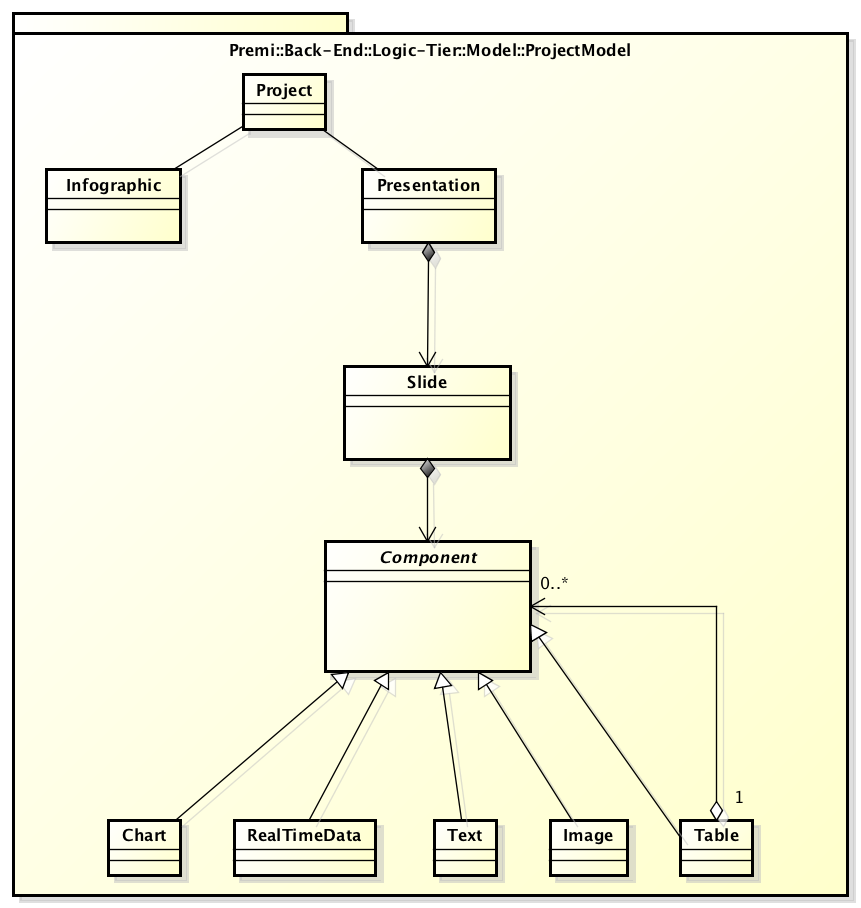
\includegraphics[width=0.9\linewidth]{img/back-end_logic-tier_model_project-model}
			\caption[Premi::Back-End::Logic-Tier::Model::ProjectModel]{Premi::Back-End::Logic-Tier::Model::ProjectModel}
		\end{figure}
		Il package contiene la struttura delle classi di tutti i componenti dell'applicazione.
	
	\subsubsection*{Classi contenute}
	\begin{itemize}
		\item Premi::Back-End::Logic-Tier::Model::ProjectModel::Project:
		\begin{itemize}
			\item \textbf{Descrizione}: classe base contenente le informazioni principali del progetto.
		\end{itemize}
			
		\item Premi::Back-End::Logic-Tier::Model::ProjectModel::Infographic:
		\begin{itemize}
			\item \textbf{Descrizione:} classe che rappresenta le infografiche associate a un progetto;
			\item \textbf{Relazione con altre classi}:
			\begin{itemize}
				\item Premi::Back-End::Logic-Tier::Model::ProjectModel::Project.
			\end{itemize}
		\end{itemize}
		
		\item Premi::Back-End::Logic-Tier::Model::ProjectModel::Presentation:
		\begin{itemize}
			\item \textbf{Descrizione:} classe che rappresenta la presentazione del progetto;
			\item \textbf{Relazione con altre classi}:
			\begin{itemize}
				\item Premi::Back-End::Logic-Tier::Model::ProjectModel::Project.
			\end{itemize}
		\end{itemize}
		
		\item Premi::Back-End::Logic-Tier::Model::ProjectModel::\gls{Slide}:
		\begin{itemize}
			\item \textbf{Descrizione:} classe che rappresenta le \gls{slide} che compongono una presentazione;
			\item \textbf{Relazione con altre classi}:
			\begin{itemize}
				\item Premi::Back-End::Logic-Tier::Model::ProjectModel::Project.
			\end{itemize}
		\end{itemize}
		
		\item Premi::Back-End::Logic-Tier::Model::ProjectModel::Component:
		\begin{itemize}
			\item \textbf{Descrizione:} classe base che rappresenta i componenti di cui è formata una \gls{slide};
			\item \textbf{Relazione con altre classi}:
			\begin{itemize}
				\item Premi::Back-End::Logic-Tier::Model::ProjectModel::Project.
			\end{itemize}
		\end{itemize}
		
		\item Premi::Back-End::Logic-Tier::Model::ProjectModel::Chart:
		\begin{itemize}
			\item \textbf{Descrizione:} classe che rappresenta l'elemento "grafico" che può essere inserito in una \gls{slide};
			\item \textbf{Relazione con altre classi}:
			\begin{itemize}
				\item Premi::Back-End::Logic-Tier::Model::ProjectModel::Project.
			\end{itemize}
		\end{itemize}
		
		\item Premi::Back-End::Logic-Tier::Model::ProjectModel::RealTimeData:
		\begin{itemize}
			\item \textbf{Descrizione:} classe che rappresenta l'elemento "dati real-time" che può essere inserito in una \gls{slide};
			\item \textbf{Relazione con altre classi}:
			\begin{itemize}
				\item Premi::Back-End::Logic-Tier::Model::ProjectModel::Project.
			\end{itemize}
		\end{itemize}
		
		\item Premi::Back-End::Logic-Tier::Model::ProjectModel::Text:
		\begin{itemize}
			\item \textbf{Descrizione:} classe che rappresenta l'elemento "testo" che può essere inserito in una \gls{slide};
			\item \textbf{Relazione con altre classi}:
			\begin{itemize}
				\item Premi::Back-End::Logic-Tier::Model::ProjectModel::Project.
			\end{itemize}
		\end{itemize}
		
		\item Premi::Back-End::Logic-Tier::Model::ProjectModel::Image:
		\begin{itemize}
			\item \textbf{Descrizione:} classe che rappresenta l'elemento "immagine" che può essere inserito in una \gls{slide};
			\item \textbf{Relazione con altre classi}:
			\begin{itemize}
				\item Premi::Back-End::Logic-Tier::Model::ProjectModel::Project.
			\end{itemize}
		\end{itemize}
		
		\item Premi::Back-End::Logic-Tier::Model::ProjectModel::Table:
		\begin{itemize}
			\item \textbf{Descrizione:} classe che rappresenta l'elemento "tabella" che può essere inserito in una \gls{slide};
			\item \textbf{Relazione con altre classi}:
			\begin{itemize}
				\item Premi::Back-End::Logic-Tier::Model::ProjectModel::Project.
			\end{itemize}
		\end{itemize}
	\end{itemize}

\newpage

\subsection{Premi::Back-End::Data-Tier}
	\subsubsection*{Informazioni sul package}
		\begin{figure}[h]
			\centering
			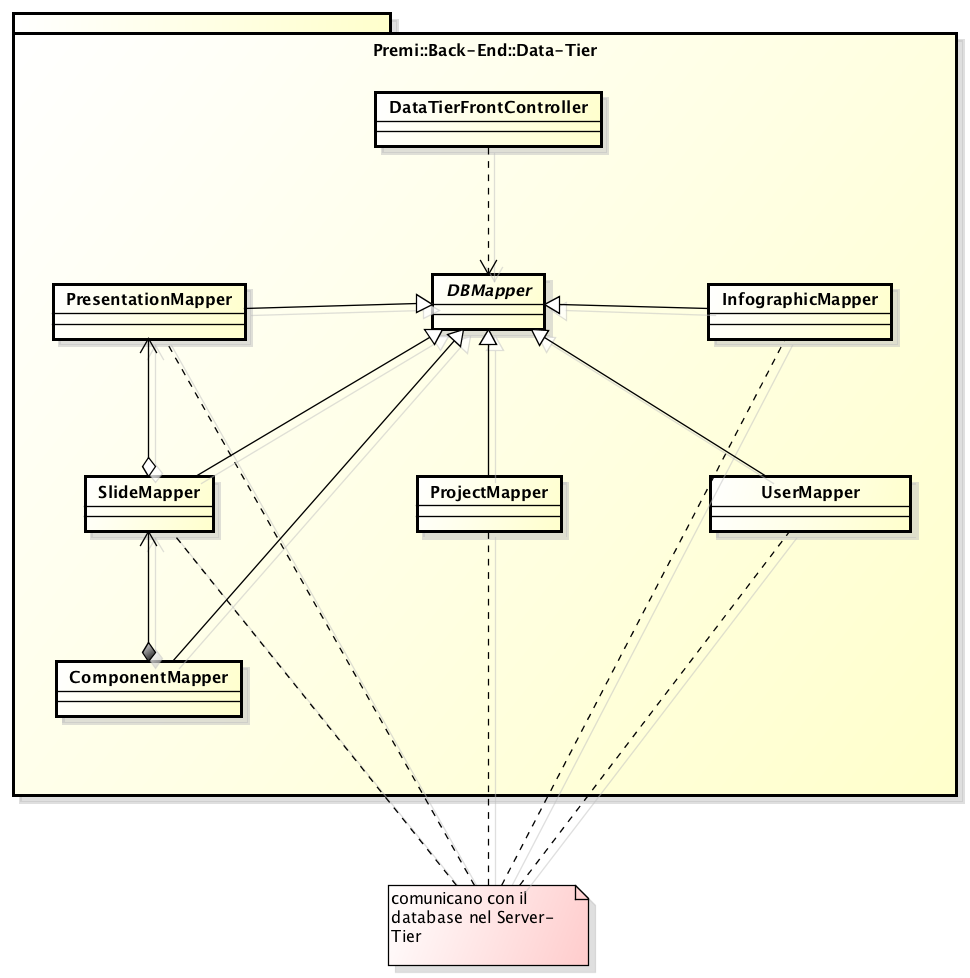
\includegraphics[width=0.9\linewidth]{img/back-end_data-tier}
			\caption[Premi::Back-End::Data-Tier]{Premi::Back-End::Data-Tier}
		\end{figure}
		Il package contiene le componenti che gestiscono l'interazione con il tier per la gestione dei dati consistenti.
		
		\subsubsection*{Classi contenute}
		\begin{itemize}
			\item Premi::Back-End::Data-Tier::DataTierFrontController:
				\begin{itemize}
					\item \textbf{Descrizione}: classe per interagire con il livello superiore e ricevere i dati dal model;
					\item \textbf{Relazione con altre classi}:
					\begin{itemize}
						\item Premi::Back-End::Logic-Tier::Model::ProjectModel::MongoHandler.
					\end{itemize}
				\end{itemize}
			
			\item Premi::Back-End::Data-Tier::DataTierFrontController:
				\begin{itemize}
					\item \textbf{Descrizione}: classe per interagire con il livello superiore e ricevere i dati dal model;
					\item \textbf{Relazione con altre classi}:
					\begin{itemize}
						\item Premi::Back-End::Logic-Tier::Model::ProjectModel::MongoHandler;
						\item Premi::Back-End::Data-Tier::DBMapper.
					\end{itemize}
				\end{itemize}
				
			\item Premi::Back-End::Data-Tier::ProjectMapper:
			\begin{itemize}
				\item \textbf{Descrizione}: classe mapper per il caricamento e il salvataggio di oggetti di tipo progetto nel \gls{database}.
				\item \textbf{Relazione con altre classi}:
				\begin{itemize}
					\item Premi::Back-End::Data-Tier::DBMapper.
				\end{itemize}
			\end{itemize}
				
			\item Premi::Back-End::Data-Tier::PresentationMapper:
			\begin{itemize}
				\item \textbf{Descrizione}: classe mapper per il caricamento e il salvataggio di oggetti di tipo presentazione nel \gls{database}.
				\item \textbf{Relazione con altre classi}:
				\begin{itemize}
					\item Premi::Back-End::Data-Tier::DBMapper.
				\end{itemize}
			\end{itemize}
			
			\item Premi::Back-End::Data-Tier::SlideMapper:
			\begin{itemize}
				\item \textbf{Descrizione}: classe mapper per il caricamento e il salvataggio di oggetti di tipo \gls{slide} nel \gls{database}.
				\item \textbf{Relazione con altre classi}:
				\begin{itemize}
					\item Premi::Back-End::Data-Tier::DBMapper.
				\end{itemize}
			\end{itemize}
			
			\item Premi::Back-End::Data-Tier::ComponentMapper:
			\begin{itemize}
				\item \textbf{Descrizione}: classe mapper per il caricamento e il salvataggio di oggetti componenti della \gls{slide} nel \gls{database}. Da questa classe deriveranno le altre classi specifiche per ogni componente, seguendo la struttura descritta all'interno del package *::ProjectModel;
				\item \textbf{Relazione con altre classi}:
				\begin{itemize}
					\item Premi::Back-End::Data-Tier::DBMapper.
				\end{itemize}
			\end{itemize}
			
			\item Premi::Back-End::Data-Tier::InfographicMapper:
			\begin{itemize}
				\item \textbf{Descrizione}: classe mapper per il caricamento e il salvataggio di oggetti di tipo \gls{infografica} nel \gls{database}.
				\item \textbf{Relazione con altre classi}:
				\begin{itemize}
					\item Premi::Back-End::Data-Tier::DBMapper.
				\end{itemize}
			\end{itemize}
			
			\item Premi::Back-End::Data-Tier::UserMapper:
			\begin{itemize}
				\item \textbf{Descrizione}: classe mapper per il caricamento e il salvataggio di oggetti di tipo utente nel \gls{database}.
				\item \textbf{Relazione con altre classi}:
				\begin{itemize}
					\item Premi::Back-End::Data-Tier::DBMapper.
				\end{itemize}
			\end{itemize}
		\end{itemize}
